%%%%
\documentclass[12pt,a4paper]{report}

% packages...
\usepackage[utf8]{inputenc}
\usepackage[english,italian]{babel}
\usepackage[hyphens]{url}
\usepackage{csquotes}
\usepackage{caption}
\usepackage{subcaption}
% Per generare il file PDF aderente alle specifiche PDF/A-1b. Verificarne poi la validità.
%\usepackage[a-1b]{pdfx}

\usepackage{hyperref}
\usepackage{graphicx}
\graphicspath{ {Img/} }
\usepackage{lipsum}% Per inserire testo a caso in attesa di realizzare i capitoli
\usepackage{listings}
\usepackage{epigraph} % per le frasi inizio capitolo
\usepackage{fancyhdr}
% \usepackage{refcheck}

\usepackage{pgfplots} 
\pgfplotsset{compat=1.18} 


\lstset{
	% 	language=bash
	frame=single,
	breaklines=true,
	postbreak=\raisebox{0ex}[0ex][0ex]{\ensuremath{\color{red}\hookrightarrow\space}},
	basicstyle=\ttfamily\footnotesize
}


%MyStyle
\renewcommand{\lstlistingname}{Code}

\definecolor{codegray}{rgb}{0.5,0.5,0.5}
\definecolor{codepurple}{rgb}{0.58,0,0.82}
\definecolor{backcolour}{rgb}{0.95,0.95,0.92}

\lstdefinestyle{Cstyle}{
    backgroundcolor=\color{backcolour},   
    keywordstyle=\color{blue},    
    numberstyle=\tiny\color{codegray},
    stringstyle=\color{codepurple},
    basicstyle=\ttfamily\footnotesize,
    breakatwhitespace=false,         
    breaklines=true,                 
    captionpos=b,                    
    keepspaces=true,                 
    numbers=left,                    
    numbersep=5pt,                  
    showspaces=false,                
    showstringspaces=false,
    showtabs=false,                  
    tabsize=2,
    frame = leftline
}

% RISC style
\lstdefinelanguage{Risc-v}
{
  alsoletter={.}, % allow dots in keywords
  alsodigit={0x}, % hex numbers are numbers too!
  morekeywords=[1]{ % instructions
    lb, lh, lw, lbu, lhu,
    sb, sh, sw,
    sll, slli, srl, srli, sra, srai,
    add, addi, sub, lui, auipc,addiw
    xor, xori, or, ori, and, andi,
    slt, slti, sltu, sltiu,
    beq, bne, blt, bge, bltu, bgeu,
    j, jr, jal, jalr, ret,
    scall, break, nop
  },
  morekeywords=[2]{ % sections of our code and other directives
    .align, .ascii, .asciiz, .byte, .data, .double, .extern,
    .float, .globl, .half, .kdata, .ktext, .set, .space, .text, .word
  },
  morekeywords=[3]{ % registers
    zero, ra, sp, gp, tp, s0, fp,
    t0, t1, t2, t3, t4, t5, t6,
    s1, s2, s3, s4, s5, s6, s7, s8, s9, s10, s11,
    a0, a1, a2, a3, a4, a5, a6, a7,
    ft0, ft1, ft2, ft3, ft4, ft5, ft6, ft7,
    fs0, fs1, fs2, fs3, fs4, fs5, fs6, fs7, fs8, fs9, fs10, fs11,
    fa0, fa1, fa2, fa3, fa4, fa5, fa6, fa7
  },
  morecomment=[l]{;},   % mark ; as line comment start
  morecomment=[l]{\#},  % as well as # (even though it is unconventional)
  morestring=[b]",      % mark " as string start/end
  morestring=[b]'       % also mark ' as string start/end
}

\lstset{
  % listings sonderzeichen (for german weirdness)
  literate={ö}{{\"o}}1
           {ä}{{\"a}}1
           {ü}{{\"u}}1,
  basicstyle=\tiny\ttfamily,                    % very small code
  breaklines=true,                              % break long lines
  commentstyle=\itshape\color{green!50!black},  % comments are green
  keywordstyle=[1]\color{blue!80!black},        % instructions are blue
  keywordstyle=[2]\color{orange!80!black},      % sections/other directives are orange
  keywordstyle=[3]\color{red!50!black},         % registers are red
  stringstyle=\color{mauve},                    % strings are from the telekom
  identifierstyle=\color{teal},                 % user declared addresses are teal
  frame=l,                                      % black line on the left side of code
  language=Risc-v,                   % all code is RISC-V
  tabsize=4,                                    % indent tabs with 4 spaces
  showstringspaces=false                        % do not replace spaces with weird underlines
}

%--- BIBIOGRAFIA
 \usepackage[ backend=biber, 
sorting=ynt,
%citestyle=authoryear 
]{biblatex}

\addbibresource{Bibliografia.bib}
%---

\usepackage[textwidth=2cm, textsize=scriptsize,colorinlistoftodos]{todonotes}
\setlength {\marginparwidth }{2cm}
%\usepackage[disable]{todonotes}

%%%%%%%%%%%%%%%%%%%%%%%%%%%%%%%%%%%%%%%%%%%%%%%%%%%%%
\begin{document}
% Frontespizio
\begin{titlepage}
\begin{center}

\includegraphics[width=\textwidth]{Img/Logo.jpg}\\
{\large{\bf Corso di Laurea Informatica}}
\end{center}
\vspace{12mm}
\begin{center}

\vspace{4mm}
{\huge{\bf RISC-V stress testing}}\\
\vspace{4mm}

\end{center}
\vspace{12mm}
\begin{flushleft}
{\large{\bf Relatore:}}
{\large{Trentini Andrea}}\\
\vspace{4mm}
{\large{\bf Correlatore:}}
{\large{Carraturo Alexjan}}\\
\end{flushleft}
\vspace{12mm}
\begin{flushright}
{\large{\bf Tesi di Laurea di:}}
{\large{Bianchessi Mattia}}\\
{\large{\bf Matr. 931455}}\\
\end{flushright}
\vspace{4mm}
\begin{center}
{\large{\bf Anno Accademico 2022-2023}}
\end{center}
\end{titlepage}


\listoftodos

%%%%%%%%
\chapter*{Introduzione}

%\textbf{Oggetto della tesi}
Il processore è il componente hardware con il quale vengono svolte le istruzioni.
Oggigiorno sono presenti numerosi processori ognuno caratterizzato da un insieme di istruzioni che definiscono le istruzioni che, un processore,  può eseguire. RISC-V , con un \textit{istruction set} basato su un approccio \textit{reduced instruction set computer}, sta facendo parlare di sè.   

%\textbf{OBIETTIVI}
L'obiettivo di questa tesi è quello di fare alcuni test sul processore dotato di RISC-V e valutarne le prestazioni.

%\textbf{METODI E STRUMENTI}
Per la valutazione sono stati scrittura dei codici in linguaggio C compilati con la \textit{toolchain} di RISC-V.I risultati dei programmi vengono riportati e , in alcuni casi, comparati con risultati di programmi simili compilati per altri processori.
In alcuni casi viene anche analizzato il sorgente compilato.

%\textbf{Struttura }
La tesi inizia con una panoramica sul progetto RISC-V presentando gli obiettivi e una panoramica  sulla storia del progetto. Il capitolo successivo presenta in sintesi l' ISA di RISC-V presentando alcuni punti importanti del progetto. Successivamente viene presentati alcuni tool di compilazione utilizzati per i programmi. I capitolo 4 e 5 vengono presentati alcuni programmi utilizzati per la valutazione e analizzati i risultati ottenuti.


\tableofcontents
\listoffigures
\listoftables
\lstlistoflistings

% o sections (dipende dal documentclass)
\chapter{RISC-V}

% OUTLINE CH 1 
% ->>>>Un approccio meno giornalistico 
%	1- presentazione progetto , (1.1- obbiettivi )
%	2- storia  \\
RISC-V è una ISA basato sul principio RISC nato come progetto accademico.  Nel 2010, a Berkeley, il progetto inizio diretto dal prof. David Patterson finanziato da \textit{Intel} e \textit{Microsoft} e da alcune aziende Californiane. La prima pubblicazione è dell anno successivo. Nel 2015 viene fondata  \textbf{RISC-V Foudation} un azienda no-profit che controlla la direzione di sviluppo di RISC-V. Nel 2018 viene annunciata una collaborazione tra l'azienda e \textit{Linux Foundation} con il quale si supporta lo sviluppo del progetto RISC-V.



\section{Gli obbiettivi di RISC-V}
Durante la fase di progettazione i progettisti hanno voluto mettere nero su bianco gli obbiettivi di RISC-V. Gli obbiettivi dichiarati , nell'introduzione, della specifica dell' ISA user-mode sono:
\begin{itemize}
	\item un ISA con una licenza \textit{open source} disponibile per accademie e industria.
	\item un ISA adatta ad un’implementazione hardware diretta, non una simulazione.
	\item un ISA non specifica per una micro-architettura o una tecnologia ma che permetta un implementazione efficente per ogni implementazione.
	\item modulare , organizzata in ISA più piccole con la possibilita di usare estensioni.
	\item supporto per lo standard floating-point 2008 IEEE-754.
	\item supporto delle estensioni .
	\item spazio di indirizzamento 32 e 64 bit.
	\item supporto a delle implementazioni multicore e manycore sia ererogeneei sia omogenei.
	\item Istruzioni a lunghezza variabile.
	\item completamente virtualizzabile 
	\item permetta la semplificazione degli esperimenti con nuovi progetti ISA con \textit{supervisor-level} e \textit{hypervisor-level}. 
	
\end{itemize}

\section{Panoramica}
L'ISA RISC-V è un architettura load-store con solo 49 istruzioni base. L'ISA supporta sistemi di memoria \textit{little-endian} che \textit{big-endian}. Le istruzioni sono organizzate in pacchetti da 16-bit memorizzati in maniera \textit{little-endian} indipendentemente dall endianness del sistema.  Ogni pacchetto ha nei bit meno significativi i bit per la codifica della lunghezza in questo modo il sistema lo decodifica, in questo modo le istruzioni di lunghezza variabile sono decodificate velocemente.

Le celle della memoria principale sono di lunghezza variabile a seconda dell' ISA base scelto, il numero di celle di memoria è XLEN e la dimensione della singola cella è di $2^{XLEN - 1}$. Ad esempio l'ISA RV32I ha un XLEN di 32.Lo spazio di indirizzamento è circolare quindi l'errore di overflow non c'è in quanto i calcoli degli indirizzi vengono scalati in modo adeguato dividendo per un modulo adeguato , sfruttando dunque la caratteristica circolare.

%Modalita indirizzamento
Avendo tutte le istruzioni di lunghezza fissa non è possibile avere direttamente costanti o indirizzi superiori alla lunghezza assegnata al campo dell istruzione. La soluzione è l'utilizzo della modalità di indirizzamento
\begin{itemize}
	\item \textbf{indirizzamento immediato}, l’operando è una costante nell’istruzione è comunque limitato dai bit assegnati del campo.
	\item \textbf{indirizzamento a registro} l’operando è un registro.
	\item \textbf{indirizzamento di base con spostamento}, l’operando è la somma tra il
contenuto di un registro e una costante.
\item \textbf{indirizzamento relativo al PC} l'operando dipende dal \textit{Program Counter} che viene sommato a una costante.
\end{itemize}

Essendo un’architettura RISC e dunque avendo tutte le istruzioni a lunghezza fissa, non è possibile avere direttamente costanti o indirizzi superiori alla lunghezza assegnata al campo dell’istruzione. Per ovviare a questo problema si usano quelle che sono dette modalità di indirizzamento:

%Eccezioni, trap, iterrupt
Si parla di eccezione quando una condizione non comune avviene a \textit{run time} associata a un istruzione.
Si parla di \textit{trap} quando verifica un trasferimento di controllo, da parte del \textit{trap handler}, da un  \textit{thread} ad un altro. Si parla di \textit{interrupt} quando la situazione imprevista è qualcosa di esterno.


%%
% Capitolo 2
% BASE -> ESTENSIONI
% 
\chapter{ISA RISC-V}
Prima di discutere dei risultati ottenuti presentiamo ISA. 
%BASE ED ESTENSIONE
\section{Base}
RISC-V prevede un nucleo di istruzioni di base mediante le quali si può supportare dei sistemi funzionanti. Esistono diversi nuclei base denominati a seconda di quanti bit utilizza il sistema.  Esistono 4 basi:
\begin{itemize}
	\item RV32I, che ha lo spazio di indirizzamento di 32 bit.  
	\item RV64I, che ha lo spazio di indirizzamento di 64 bit.
	\item RV128I, che ha lo spazio di indirizzamento di 128 bit.
	\item RV32E,  sotto-insieme di RV32I che ne offre un supporto simile ed è pensata  per dispositivi embedded.
\end{itemize}
Tutte le ISA base usano il complemento a due per la rappresentazione di valori interi con segno.  Le basi per la computazione a valori interi è identificata dalla lettera "I". 

%Perche avere estensioni
%%?
\section{Estensioni}
Se si utilizza solo una base si hanno solo delle funzionalità basilari, per questo motivo vengono introdotte le estensioni. Usare un estensione significa estendere le funzionalità e aggiungere il supporto per determinate azioni.Di seguito vengono riportate alcune estensioni:
\begin{itemize}
		\item "M", aggiunge istruzioni per le operazioni di moltiplicazioni e divisioni di interi.
		\item "A" istruzioni atomiche,  istruzioni di lettura-scrittura-modifica atomiche. % Atomiche = def?
		\item "F"istruzioni a virgola mobile a singola precisione , aggiungendo anche registri, istruzioni, load e store a virgola mobile a singola precisione.
		\item "M" istruzioni a virgola mobile a doppia precisione.
		\item "C" istruzioni a 16 bit.
\end{itemize}

Le estensioni, possono essere di tre tipi in base alla standardizzazione:
\begin{itemize}
	\item \textbf{standard} definite dalla RISC-V Foundation.
	\item \textbf{reserved} non ancora definite ma riservate per usi futuri.
	\item \textbf{non standard} non definita dalla RISC-V Foundation.
\end{itemize}

\begin{table}
\centering
\begin{tabular}{|c|l|c|}
\hline
Base & Versione & Definitiva? \\
\hline
RV32I & 2.0 & S\\
RV32E & 1.9 & N\\
RV64I & 2.0 & S\\
RV128I & 1.7 & N\\
\hline
Estensione & Versione & Definitiva? \\
\hline
M & 2.0 & S\\
A & 2.0 & S\\
F & 2.0 & S\\
D & 2.0 & S\\
Q & 2.0 & S\\
L & 0.0 & N\\
C & 2.0 & S\\
B & 0.0 & N\\
J & 0.0 & N\\
T & 0.0 & N \\
P & 0.1 & N\\
V & 0.2 & N\\
N & 1.1 & N\\
\hline

\end{tabular}
	\caption{Tabella nomenclatura ISA RISC-V}
	\label{tab:nomenclaturaISA}
\end{table}

La tabella  \ref{tab:nomenclaturaISA}, presa da SPEC-2.2 \cite{ISA},  presenta i set base e le estensioni standard con le rispettive versioni. Ogni base o estensione presenta la casella ''Definitiva'' che specifica se il set o l 'estensione è definitiva (S) o non lo è (N).


\section{Istruzioni base}
Di base l'ISA presenta un piccolo insieme di istruzioni  Le istruzioni base sono solamente 47 e vengono codificate in 6 formati (R/I/S/U/B/J).  

\begin{figure}[h!]
	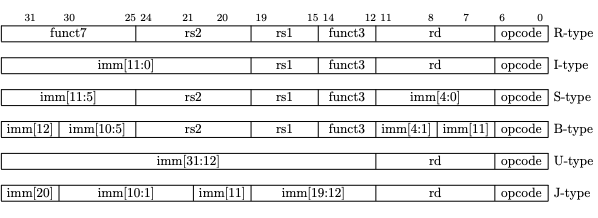
\includegraphics[width = \textwidth]{FormatiIstruzione.png}
	\caption{Formati istruzione RISC-V}
	\label{Fig:Formati_istruzioni_RV32I}
	\cite{ISA}
\end{figure}



In tutti i formati i registri sorgente (\textit{rs1} e \textit{rs2}) e il registro destinazione (\textit{rd}) vengono mantenuti nelle stesso posizioni per velocizzare la codifica.
I formati B e J possono essere visti come delle variazioni dei formati S e U nel senso che il campo imm dei formati B e J sono un ulteriore divisione dello stesso campo dei formati S e U,  ad esempio il fomato S, ha un solo campo imm compreso tra 25:31 bit per il formato B il campo è diviso in due ma mantenuto nella stessa posizione.  L'ISA presenta 4 categorie di istruzioni:
\begin{itemize}
	\item \textbf{Istruzioni computazionali}: Sono presenti 21 istruzioni computazionali e vengono codificate nel formati R se è un'operazione trai registri o nel formato I se è un'operazione tra registro e immediato. Le istruzioni di questo tipo includono istruzioni aritmetiche, logiche e di comparazione sia per valore senza segno che valori con segno.
	\item \textbf{Accesso alla memoria}Le istruzioni di accesso alla memoria premetto il trasferimento di datti dalla memoria e alla memoria. Sono presenti 8 istruzioni in totale, 5 di load codificate nel formato I e 3 di store codificate nel formato S.
	\item \textbf{Controllo del flusso}Le istruzioni di controllo permettono di alterare il normale flusso sequenziale del programma. Sono presenti 6 istruzioni di questo tipo che permettono il trasferimento codificate nel formato B. Le istruzioni prevedono il confronto degli operandi in \textit{rs1} e \textit{rs2} se la condizione  è verificate viene aggiunto il valore del campo imm al \textit{program counter} per raggiungere l'indirizzo di arrivo.
	\item \textbf{Istruzioni di sistema}Con RV32I sono presenti 8 istruzioni di controllo del sistema. Possiamo dividerle in due gruppi. Il primo gruppo (ECALL, EBREAK) gestisce  le \textit{system call}. Il secondo gruppo sono utilizzate per leggere e scrivere i registri di stato.
\end{itemize}


\section{RV32I}
L'ISA base è stata progettata per supportare i moderni sistemi operativi. Questa base contiene 47 istruzioni uniche.  I 32 registri sono di 32 bit (XLEN = 32) vengono identificati da x seguito da un numero. Il primo registro x0 contiene la costante zero e ogni istruzione che cerca di modificarlo solleva un eccezione. Gli altri registri x1 - x31 sono \textit{general purpose}.  L'ABI definisce le convenzioni di utilizzo dei registri(Figura \ref{Fig:ConvenzioneRegistri}).

\begin{figure}[h!]
\centering
	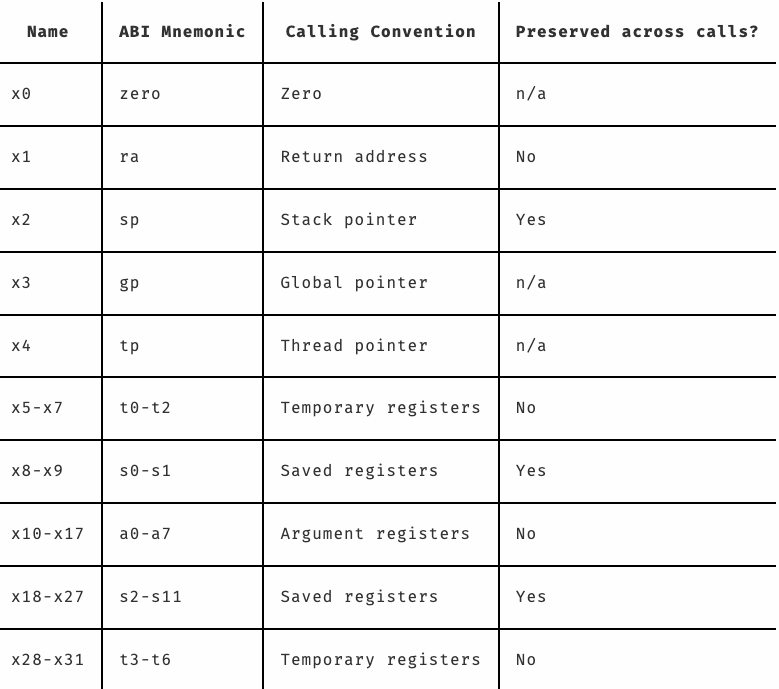
\includegraphics[scale=0.3]{ABI-RISC-V}
	\caption{Convenzione dei registri}
	\label{Fig:ConvenzioneRegistri}
\end{figure}

Come mostrato in Figura \ref{Fig:ConvenzioneRegistri} notiamo che non è presente un registro dedicato allo \textit{stack pointer} ne un \textit{return adress} ma vengono utilizzati rispettivamente il registro x2 e il registro x1.


\section{Le altre basi}
Esistono altri set che aumentano i bit utilizzati dai registri come RV64I e RV128I. Tutto cio che è stato detto è valido anche per queste con alcuni accorgimenti che sollevano eccezioni di operazioni non valide.
Rispettivamente il valore di XLEN per RV64I e per RV128I è 128.


Sul documento che propone RISC-V sul proprio ISA vengono anche impostate le linee guida per fare delle proprie estensioni.

\todo{Ho trovato i primi 2 capitoli molto più leggibili. Hai fatto bene a smaltire}




%%
%Capitolo 3: Compilatori
% cos è -> Storia -> Riguardo RISC-V  -> due parole su gcc e clang

\chapter{Compilatori}

\section{Descrizione}
Un compilatore è un programma che trasforma il codice sorgente in linguaggio macchina. Il motivo più comune per trasformare il codice sorgente è creare un programma eseguibile su una determinata macchina. Il processo di compilazione prevede diverse fasi. La prima prevede un analisi lessicale da cui vengono generati dei token. La seconda ,utilizzando i token, prevede un analisi sintattica e infine un analisi semantica dopo la quale viene generato il codice un codice intermedio. Questo codice intermedio attraversa una fase di ottimizzazione e infine viene generato il codice target.


\begin{figure}
\centering
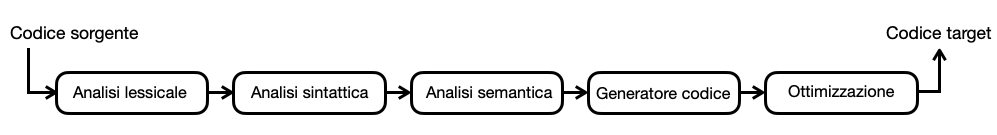
\includegraphics[width = \textwidth]{SchemaCompilatore.png}
\caption{Schema meccanismo di compilazione}
\label{Fig:MeccanismoCompilazione}
\end{figure} % figura disegnata io

Qualsiasi programma scritto in un linguaggio di programmazione di alto livello deve essere tradotto in codice oggetto prima di poter essere eseguito, quindi tutti i programmatori che utilizzano tale linguaggio utilizzano un compilatore o un interprete. I miglioramenti a un compilatore possono portare a un gran numero di funzionalità migliorate nei programmi eseguibili.

\section{Storia}
Il primo compilatore teorico fu pensato da Corrado Böhm che nel 1951 che lo sviluppò per la sua tesi di dottorato.  Una  prima implementazione di un compilatore è dovuta a Grace Hopper  che ha anche coniato il termine ``compilatore''.  Il primo compilatore , chiamato \textit{A-0 System} ,  funzionava come caricatore o linker , non come i moderni compilatori. E' importante menzionare che una versione successiva del \textit{A-0 System} (la versione A-2 datata 1953)fu rilasciato ai clienti con lo scopo di sviluppare dei miglioramenti all UNIVAC, quindi possiamo considerarlo come il primo software libero e open source della storia dell'informatica \cite{SystemA0}.


\section{Cross-compilazione}
\label{Sec:Cross}
Con il termine \textbf{Cross.compilazione} si intende la tecnica mediante la quale si utilizza un compilatore per compilare il codice sorgente e il codice generato ha come target un architettura diversa da quella su cui viene utilizzato il cross-compilatore.  Alcuni esempi di una cross-compilazione può essere la compilazione di un applicazione per un sistema embedded. 


\section{Compilatori moderni}
Nel ecosistema dei compilatori moderni i due dei piu famosi sono: GCC e CLANG.
Il primo GCC (GNU Compiler Collection) fu creato nel 1987 oggi viene sviluppato da programmatori di tutto il mondo. Inizialmente nato per il linguaggio C oggi oggi supporta altri linguaggi come Java, C++, Objective C \cite{GCCstory}.

Il secondo nato nel 2005 sviluppato da Apple Inc.  Inizialmente fu sviluppato con lo scopo di avere un compilatore Apple ottimizzato per i loro dispositivi\cite{ClangStory}.

\textit{Domanda: Ma tu hai usato CLANG?} 

\section{Un buon compilatore} %
La scelta di un compilatore per un progetto è una scelta importante.I processori, oggi, sono strutturati in pipeline supescalari e in altre complesse strutture interne. Inoltre i linguaggi moderni astraggono dalla struttura hardware per ottenere un linguaggio logico più generale. Quindi si predilige un approccio meno specifico e non incentrato sulla struttura della macchina.Gli standard dei linguaggi, si fanno  sempre più espressivi e astratti.  Questa espressività dei linguaggi aumenta l'onere dei compilatori che devono essere in grado di generare un buon codice assembly. La selezione di un compilatore è una scelta cruciale per il proprio progetto, si deve tener conto che la stessa porzione di codice, utilizzando compilatori differenti, può generare comandi assembly più o meno efficienti.
Oltre a generare programmi eseguibili ad alte prestazioni, i compilatori devono anche avere prestazioni elevate. Un progetto software di grandi dimensioni  può contenere da centinaia a migliaia di singole unità di traduzione. Ogni unità di traduzione può contenere migliaia di righe di codice.  Oltre all efficienza delle prestazioni del codice generato si deve tener conto anche del tempo in cui si genera il codice.

Quindi, un buon compilatore ci permette di concentrarci sul processo di programmazione,  piuttosto che farci preoccupare della struttura del sistema e deve essere in grado di produrre del codice che abbia delle buone performance in tempo relativamente breve.


\section{Toolchain di RISC-V}
In sistemi privi di un compilatore viene utilizzata la tecnica della \textbf{cross-compilazione}(Sezione \ref{Sec:Cross}).  RISC-V mette a disposizione alcune \textit{toolchain} di compilazione. Una \textit{toolchain} è un insieme di programmi utilizzati sequenzialmente per la creazione di un software. Per RISC-V sono disponibili le \textit{toolchain gcc}\cite{toolchain_gcc} e \textit{toolchain clang}\cite{toolchain_clang}. Entrambe le \textit{toolchain} sono mantenute dalle community, quella piu aggiornata e utilizzata è quella del progetto GNU.  Sul \href{https://wiki.riscv.org/display/HOME/RISC-V+Software+Ecosystem}{sito} sono elencate tutte le \textit{toolchain} disponibili ma anche offre una panoramica su tutto l'ecosistema RISC-V.


\subsubsection{GCC toolchain}
La toolchain GCC di RISC-V supporta linguaggi come C, C++, Objective-C,e Go. La versione corrente è la 12.2 (datata Agosto 2022).  La toolchain ha aggionamenti molto di frequente.  Ci sono quattro manutentori Andrew Waterman,Jim Wilson, Kito Cheng, Palmer Dabbelt .

\subsubsection{CLANG toolchain}
La toolchain LLVM/CLANG è sviluppata da \textit{lowRISC project} attualmente è alla versione 15.0.2. A differenza della \textit{toolchain gcc} è mantenuta solamente da Alex Bradbury.


%%%--------------------

\chapter{BenchMarking}
\section{Descrizione board}

La scheda di sviluppo utilizzata è  D1-H Nezha basata sul design del chip Allwinner D1-H. La board integra una CPU Ali Pingtou Ge RISC-V C906, con clock a 1 GHz, supporta il kernel Linux standard, supporta  2G DDR3, 258 MB di spin-nand, WiFi/Bluetooth connessione, con interfacce audio e video,  può essere collegato a varie periferiche, interfaccia MIPI-DSI+TP integrata, interfaccia scheda SD,interfaccia HDMI, interfaccia scheda figlia microfono, interfaccia auricolari da 3,5 mm , interfaccia Gigabit Ethernet, USB HOST, interfaccia di tipo C, interfaccia di debug UART, array di pin a 40 pin.

\begin{figure}[!ht]
\includegraphics[width = \textwidth]{D1H-BoardTopView.png}
\caption{Board vista dall' alto}

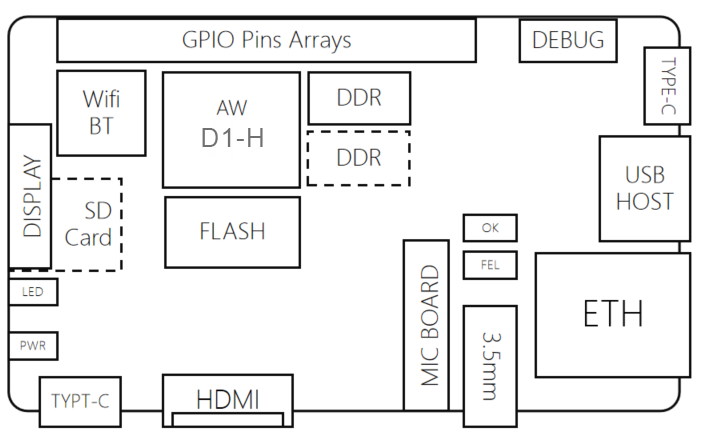
\includegraphics[width = \textwidth]{D1H-BoardBlockView.png}
\caption{Schema a blocchi della scheda di sviluppo}\cite{BoardInfo}
\end{figure}

\vspace{2cm}

\begin{table}[!ht]
\centering
\begin{tabular}{| r | c |}
\hline
CPU & Allwinner D1-H \\
\hline
Clock & 1GHz\\
\hline
DRAM & DDR3 2GB\\
\hline
Memoria & 256MB  spin-nand integrato\\
\hline 
Supporto memoria & USB e  SD\\
\hline
Rete & Gigabit Ethernet,  2.4G WiFi e Bluetooth , antenna integrata\\
\hline
Display & MIPI-DSI + TP, HDMI, SPI \\
\hline
Audio & jack per cuffie da 3,5 mm\\
\hline
Tasti & FEL, LRADC OK\\
\hline
Luci &  alimentazione, LED tricolore\\
\hline
DEBUG & UART, USB ADB\\
\hline
USB & USB , USB OTG, USB2.0\\
\hline
PIN & array di pin 40\\
\hline
Alimentazione & USB-C  5V-2A\\
\hline
Dimensioni & lunghezza 85 mm, larghezza 56 mm, spessore 1,7 mm\\
\hline

\end{tabular}
\caption{Caratteristiche della board}
\end{table}

\section{Ambiente di sviluppo}
La scheda di sviluppo D1-H viene fornita con il sistema Tina Linux. Il kernel fornito  adattato al kernel Linux 5.4. La board fornisce il supporto di base e gestione delle risorse hardware del dispositivo. Ulteriori informazioni sono disponibili sul sito della \href{https://d1.docs.aw-ol.com/study/study_1tina/}{board}.

\section{Presentazione programmi}
I programmi utilizzati sono scritti in C e sono contenuti su github in una \href{https://github.com/MattiaBianchessi/Testing_RISC-V}{repository}.
 Ogni directory contiene i dati di esecuzione di ciascun programma eseguito in un file con estensione .csv e un notebook jupyter per visualizzare i dati e, in alcuni casi, confrontarli.
\subsection{Operazioni Aritmetiche}
Il primo programma utilizzato esegue le operazioni aritmetiche di base addizione, sottrazione, moltiplicazione, divisione e modulo.
Il programma genera due matrici quadrate di numeri interi su cui vengono eseguite le operazioni elemento per elemento. Le dimensioni delle matrici sono 1000 x 1000, 2500 x 2500, 5000 x 5000, 8000 x 8000, 10000 x 10000, 15000 x 15000.

La prima matrice generata ha valori tra uno e duecento, la seconda ha valori tra uno e cento.

Per ogni matrice vengono eseguite cinque prove da cui viene calcolato il tempo medio di esecuzione.

\subsection{Prime Number}
Il programma generai primi cinquemila numeri primi. 
Il programma ''prime.c'' controlla da due in poi se n-esimo numero è divisibile se non è divisibile allora lo memorizzo altrimenti passo al prossimo numero.  

\subsection{Moltiplicazione o shift}
Il programma confronta la velocità di esecuzione di moltiplicazione e divisione aritmetiche con lo shift. Il programma genera un array di interi di valori tra zero e maxInt e un array di potenze di due comprese tra due e milleventiquattro. Entrambi gli array hanno mille elementi. Dopo la generazione viene calcolato elemento per elemento il risultato e viene memorizzato il tempo di esecuzione. Il risultato del programma è il tempo medio di esecuzione di mille operazioni per tipo (moltiplicazione normale, divisione normale, moltiplicazione tramite shift, divisione tramite shift).

\subsection{Montecarlo Pi}
Algoritmo di approssimazione del pigreco tramite il metodo di Montecarlo. Nell' esecuzione vengono utilizzati da 10 a ($ 10^{10} $) punti per l'approssimazione. Ogni iterazione viene eseguita cinque volte e per ogni iterazione viene memorizzato il valore calcolato con il proprio tempo di esecuzione. Il programma si basa sulla funzione rand.

\subsection{Sorting}
In questa directory sono presenti alcuni alcuni algoritmi di sorting. Gli algoritmi di sorting utilizzati sono:
\begin{itemize}
	\item BubbleSort
	\item InsertionSort
	\item QuickSort
	\item HeapSort
\end{itemize}

Ogni algoritmo viene eseguito su array di dimensione diversa 500, 1000, 5000, 10000, 20000, 35000, 50000. Per ogni dimensione vengono eseguite 150 prove sulle quali viene calcolato il tempo di esecuzione. Il programma informa per ogni gruppo di array il tempo massimo, il minimo e il tempo medio. Per alcuni algoritmi vengono utilizzate anche delle configurazioni particolari dell' array da ordinare, come ad esempio utilizzando il BubbleSort vengono ordinati array strettamente crescenti e strettamente decrescenti oltre che ai campioni casuali. Nella situazione generale gli array vengono generati con numeri interi casuali.

\subsection{BackTracking}
In questa directory sono contenuti due programmi che utilizzano metodi di backtracking:
\begin{itemize}
	\item Un solutore di sudoku
	\item Un solutore di labirinti
\end{itemize}

In entrambi i casi vengono utilizzate tecniche di backtracking.  Lo scopo è quello di valutare il tempo di esecuzione di programmi che fanno uso del backtracking su processore RISC.

\vspace{0.5cm}
\begin{large}
\textbf{Sudoku}
\end{large}

Il solutore di sudoku risolve il puzzle matematico.  Sono presenti otto sudoku nel file sudoku.h di varia difficoltà, 2 di essi non sono fattibili, uno per costruzione(sbagliato in partenza) e l 'altro è impossibile risolverlo per la configurazione.

\vspace{0.5cm}
\begin{large}
\textbf{MazeSolver}
\end{large}

Il solutore mazeSolver.c, una volta in esecuzione, chiede il path del labirinto da risolvere e successivamente è possibile salvare la soluzione, se trovata, in un nuovo file.  Sono presenti alcuni esempi nella sottodirectory maze di labirinti.
In directory è presente un ulteriore file mazeGen.py che è stato utilizzato come generatore di labirinti. 
Inoltre viene fornita la possibilità di utilizzare un proprio labirinto, il labirinto personale dovrà avere l'estensione .txt specificare il numero di linee e il numero di colonne del labirinto sulle prime due righe. Successivamente  il labirinto. Le componenti del labirinto sono i muri , indicati con \#, un inizio , indicato con 'I' e una fine con 'O'. Le zone dello attraversabili sono idenficate dallo spazio ' '.



\chapter{Comparativa}

\section*{MacBook Air}
\label{sec:MacBook}
Per alcuni benchmark è stato utilizzato un MacBook Air per confronto.  Il PC ha un processore 2,2 GHz Intel Core i7 dual-core con memoria 8 GB 1600 MHz. Nelle sezioni successive i termini Pc fanno riferimento a questa architettura.

\section{Operazioni}
	Con il programma operazioni viene visualizzato il tempo di esecuzione di alcune operazioni matematiche di base. Come mostrato nelle porzioni di codice Code \ref{Code:Sum},\ref{Code:Sub}, \ref{Code:Mul}, \ref{Code:Div}, \ref{Code:Mod} mostrano le funzioni che si occupano delle operazioni. Ogni funzione, semplicemente, esegue un ciclo su ogni elemento di \textit{a} e di \textit{b}, ne esegue l'operazione e memorizza il risultato in \textit{c}.  La matrice \textit{a} ha valori interi compresi tra uno e duecento,  la matrice \textit{b} ha valori interi compresi tra uno e cento. Le matrici utilizzate sono matrici quadrate e le dimensioni utilizzate sono 1000, 2500, 5000, 8000, 10000, 15000. Per ogni operazione vengono eseguite cinque prove da cui viene calcolato il tempo medio di esecuzione. 
	Per riferimento il programma è stato utilizzato anche sul Pc \ref{sec:MacBook}. 
	
	\lstinputlisting[language=c,  style = Cstyle, caption = Addizione,  label ={Code:Sum} ]{PorzioniCodice/Operazioni/sum.c}
	\lstinputlisting[language=c,  style = Cstyle, caption = Sottrazione, label ={Code:Sub}]{PorzioniCodice/Operazioni/sub.c}
	\lstinputlisting[language=c,  style = Cstyle, caption = Moltiplicazione, label ={Code:Mul}]{PorzioniCodice/Operazioni/mul.c}
	\lstinputlisting[language=c,  style = Cstyle, caption = Divisione, label ={Code:Div}]{PorzioniCodice/Operazioni/div.c}
	\lstinputlisting[language=c,  style = Cstyle, caption = Modulo, label ={Code:Mod}]{PorzioniCodice/Operazioni/mod.c}
	
	Di seguito vengono riportati i tempi di esecuzione medi per operazione e per dimensione
	\begin{table}[!ht]
	
	\centering
	\begin{tabular}{| l | c | c | c | c | c | c |}
		\hline
		Operazione & 1000 & 2500 & 5000 & 8000 & 10000 & 15000 \\ \hline
		Somma & 0.002317 & 0.013848 & 0.055129 & 0.142010 & 0.227784 & 0.504650\\ \hline
		Sottrazione & 0.002324 & 0.013921 & 0.054900 & 0.142941 & 0.227505 & 0.504767\\ \hline
		Prodotto & 0.002344 & 0.014010 & 0.055036 & 0.143293 & 0.226141 & 0.504829\\ \hline
		Divisione & 0.002352 & 0.013953 & 0.055298 & 0.142226 & 0.227948 & 0.505007\\ \hline
		Modulo & 0.002298 & 0.013880 & 0.055009 & 0.142129 & 0.227835 & 0.505035\\ \hline

	\end{tabular}
	
	\caption{Tempi di esecuzione MacBook-Air}
	\end{table}
	
	\begin{table}[!ht]
		\centering
		\begin{tabular}{{| l | c | c | c | c | c | c |}}
			\hline
			Operazione & 1000 & 2500 & 5000 & 8000 & 10000 & 15000   \\ \hline	
			Somma & 0.011256 & 0.069917 & 0.279804 & 0.714786 & 1.117411 & 2.512942  \\ \hline	
			Sottrazione & 0.011237 & 0.069850 & 0.279895 & 0.714680 & 1.117352 & 2.512978  \\ \hline	
			Prodotto & 0.011234 & 0.069899 & 0.279219 & 0.715381 & 1.117296 & 2.514183  \\ \hline	
			Divisione & 0.011170 & 0.069781 & 0.279884 & 0.714673 & 1.116763 & 2.513539  \\ \hline	
			Modulo & 0.011212 & 0.069845 & 0.279913 & 0.715371 & 1.117348 & 2.514198  \\ \hline	
		\end{tabular}
		
	\caption{Tempi di esecuzione RISC-V}
	\end{table}
	Di seguito i grafici rappresentativi delle tabelle precedenti.
	\begin{figure}
	\centering
		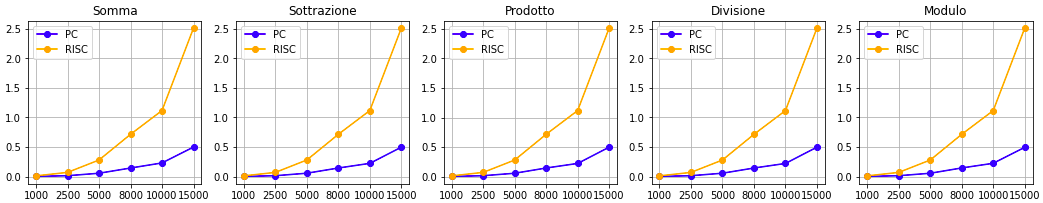
\includegraphics[scale= 0.4]{PorzioniCodice/Operazioni/Grafico.png}
	\end{figure}
	
	Prendiamo in considerazione l'operazione di somma del processore RISC. Il tempo di esecuzione per la matrice 1000 x 1000 è di 0.011256 e per la matrice 2500 x 2500 è di  0.069917 il che è 6.2115 (circa) il tempo di esecuzione e 6.25 la dimensione dei dati.  Per il Pc il tempo di esecuzione per la matrice 1000 x 1000 è di 0.002317 e per la matrice 2500 x 2500 è di  0.013848 il che è 5.97 (circa) il tempo di esecuzione e 6.25 la dimensione dei dati.  
	Il tempo di esecuzione totale del programma è di 23.653595 per il Pc mentre 117.665045 per RISC. Quindi il MacBook è 4.97 \% piu veloce del processore RISC. %risultato abbastanza prevedibile. 
	
	
\section{PrimeNumber}
Il programma utilizza una scansione lineare per trovare i primi cinquemila numeri primi. In seguito viene mostrato il codice della funzione principale.  La funzione controlla dal numero due in avanti se il numero è primo, se lo è viene inserito nell' array altrimenti no e il ciclo viene eseguito fino a trovare cinquemila numeri primi.  

\lstinputlisting[language=c,  style = Cstyle, caption = Impostazioni dei dati,  label ={Code:prime} ]{PorzioniCodice/Prime/prime.c}

I file sono stati compilato con diverse livelli di ottimizzazione.
\begin{table}[ht]
\begin{tabular}{|l|c|r|}
\hline
    & PC       & RISC-V    \\ \hline
-O2 & 0.041286 & 0.434372  \\ \hline
-O1 & 0.033024 & 0.346976  \\ \hline
-O0 & 0.032363 & 0.3122784 \\ \hline
\end{tabular}
\caption{Tempi di esecuzione numeri primi}
\label{Tab:TempoPrime}
\end{table}
Come precedentemente notato è l'ordine di grandezza di differenza dei due processori. Andando a guardare nei sorgenti assembly notiamo delle differenze. La prima abbastanza ovvia è la dimensione del file che nel caso del' ottimizzazione 0 è superiore (172 linee 4KB) rispetto all livello 2 (130 linee 4KB).Il secondo è l'utilizzato dell'istruzione \textit{nop} nel livello 0.
Il codice \ref{Code:primeO0} fa riferimento alla porzione di codice dove vengono utilizzate le istruzioni \textit{nop}.

\lstinputlisting[language = Risc-v,  caption =Sorgente prime ottimizzato con -O0,  label ={Code:primeO0},  firstline=48,lastline=55 ]{PorzioniCodice/Prime/prime0.s}

La pseudo-istruzione \textit{nop}(No operation) ha come implementazione addi x0, x0, 0 che somma zero (costante) al registro contenente zero (x0) e lo memorizza nel registro x0.  Questo è un caso eccezionale in cui si ha la possibilità di scrivere il registro x0, seppur con poco significato algebricamente, ogni altro caso in cui si vuole modificare il registro x0 solleverebbe errori. La motivazione della presenza di queste operazioni è dovuto alla struttura hardware dotata di interlock. % un fatto piu storico
La maggior parte delle implementazioni hardware ha degli interlock. Se un'istruzione necessita di dati che non sono ancora disponibili, la pipeline si interrompe finché i dati non sono disponibili. Oppure, se si tratta di una pipeline di esecuzione fuori ordine, un'istruzione si blocca finché i dati non sono disponibili e altre istruzioni possono continuare l'esecuzione.
I nop emessi dal compilatore con -O0  non vengono emessi a -O1 o superiore. 


\section{MultOrShift}
Il programma confronta la velocità di esecuzione di moltiplicazione e divisione aritmetiche con lo shift. Il programma genera un array di interi di valori tra zero e maxInt e un array di potenze di due comprese tra due e milleventiquattro. Entrambi gli array hanno mille elementi. Dopo la generazione viene calcolato elemento per elemento il risultato e viene memorizzato il tempo di esecuzione. Il risultato del programma è il tempo medio di esecuzione di mille operazioni per tipo (moltiplicazione normale, divisione normale, moltiplicazione tramite shift, divisione tramite shift). Di seguito alcune porzioni di codice:

\lstinputlisting[language=c,  style = Cstyle, caption = Impostazioni dei dati,  label ={Code:Init} ]{PorzioniCodice/MultShift/init.c}
\lstinputlisting[language=c,  style = Cstyle, caption = Impostazioni dei dati,  label ={Code:Mult} ]{PorzioniCodice/MultShift/Mult.c}
\lstinputlisting[language=c,  style = Cstyle, caption = Impostazioni dei dati,  label ={Code:Shift} ]{PorzioniCodice/MultShift/Shift.c}

Il codice \ref{Code:Init} imposta i due array.  I codici \ref{Code:Mult} e \ref{Code:Shift} mostrano l'operazione eseguita.
La tabella \ref{Tab:tempi_esecuzioneMS} mostra i tempi di esecuzione calcolati in millisecondi delle varie operazioni.

\begin{table}[ht]
\centering
\begin{tabular}{lcccc}
\cline{2-5}
\multicolumn{1}{l|}{}         & \multicolumn{2}{c|}{PC}                                   & \multicolumn{2}{c|}{RISC-V}                               \\ \hline
\multicolumn{1}{|l|}{Normale} & \multicolumn{1}{c|}{0.0036} & \multicolumn{1}{c|}{0.0042} & \multicolumn{1}{c|}{0.0430} & \multicolumn{1}{c|}{0.0572} \\ \hline
\multicolumn{1}{|l|}{Shift}   & \multicolumn{1}{c|}{0.0034} & \multicolumn{1}{c|}{0.0034} & \multicolumn{1}{c|}{0.0404} & \multicolumn{1}{c|}{0.0826} \\ \hline
                              & \multicolumn{1}{l}{}        & \multicolumn{1}{l}{}        & \multicolumn{1}{l}{}        & \multicolumn{1}{l}{}       
\end{tabular}
	\caption{Tempi di esecuzione operazioni calcolati in ms}
	\label{Tab:tempi_esecuzioneMS}
\end{table}
	
	
\section{Analisi codice assembly}
Osserviamo i compilatori a confronto.  I Compilatori confrontati sono \textit{gcc RISC-V},  \textit{gcc ARM} e \textit{gcc x86\_64}.  I compilatori RISC-V e ARM vengono confrontati per il loro focus sul ambiente embedded ed entrambi sono architetture RISC.Tutti i codici presentati in questa sezione vengono compilati e presentati con il livello di ottimizzazione di default (-O0).


\section{Operazioni}
\subsection{Addizione con costante}

\lstinputlisting[language=c,  style = Cstyle,  caption = Addizione, label = {Code:AddComp}]{PorzioniCodice/ConfrontoCompilatori/C/get_num.c}

La funzione è una semplice funzione scritta in C che dato un numero di tipo intero restituisce il numero sommato a ventitré. 

\vspace{0.3 cm}
\textbf{RISC-V}

\vspace{0.3 cm}
Il sorgente compilato con il compilatore RISC-V \ref{Code:AddRISCV} da riga due fino a riga sei predispone la chiamata della procedura posizionando sullo stack il necessario, da riga sette inizia la funzione. Su quella riga viene recuperato il valore di \textit{num} che alla riga otto, tramite l'operazione di add immediate, viene sommato a num. Il risultato dell operazione addiw è la somma del valore di num sommato alla costante ventitré, il risultato è esteso su sessantaquattro bit, vengono ignorati gli errori di overflow. Successivamente tramite la pseudo istruzione sext.w che prende i 32 bit inferiori e li memorizza nel registro rd.  Questa istruzione corrisponde a addiw rd, rs,1 0. Il risultato viene spostato nel registro a0 che, nei processori RISC-V, viene utilizzato come restituzione di risultato. Le righe successive ripristinano lo stack e restituisce il controllo al chiamante.

\vspace{0.3 cm}
\textbf{ARM}

\vspace{0.3 cm}

l sorgente  \ref{Code:Addx86} , compilato con gcc ARM, mostra che la preparazione della procedure si esegue da riga due a riga cinque, le con le due righe successive si esegue la funzione. La riga sei recupera il valore di num la riga successiva calcola il valore del risultato e, infine, alla riga otto si sposta il risultato nel registro di restituzione


\vspace{0.3 cm}
\textbf{x86}

l sorgente  \ref{Code:AddARM} è compilato con gcc di x86.  Da riga due fino a riga quattro viene preparato lo stack, a riga cinque viene posizionato num nel registro eax che a riga sei viene sommato a ventitré che viene memorizzato nel registro eax. Infine viene ridato il controllo al chiamante.

\vspace{0.3 cm}

\begin{figure}[ht]
     
     \begin{subfigure}{0.3\textwidth}
  
        \lstinputlisting[language = Risc-v, caption = {RISC-V}, label = {Code:AddRISCV} ]{PorzioniCodice/ConfrontoCompilatori/Assembler/RISC-V/get_num.txt}


     \end{subfigure}
     \hfill
     \begin{subfigure}{0.3\textwidth}
         
          \lstinputlisting[language = Risc-v, caption = {Arm}, label = {Code:AddARM}]{PorzioniCodice/ConfrontoCompilatori/Assembler/ARM/get_num.txt}


     \end{subfigure}
     \hfill
     \begin{subfigure}{0.3\textwidth}
         
          \lstinputlisting[language = Risc-v, caption = {x86}, 	label = {Code:Addx86}]{PorzioniCodice/ConfrontoCompilatori/Assembler/x86/get_num.txt}


     \end{subfigure}
    
        \caption{Funzione di somma}
        
\end{figure}

\subsection{Addizione}
Nel caso generale viene calcolata la somma di tre numeri.
\lstinputlisting[language=C,  style = Cstyle,  caption = {Addizione generale}, label = {Code:Add2Comp}]{PorzioniCodice/ConfrontoCompilatori/C/sumGen.c}


\vspace{0.3 cm}
\textbf{RISC-V}

Nel caso del compilatore RISC-V la somma avviene tra tredici e diciannove dove gli operandi vengono caricati nei registri a4 e a5,  successivamente calcolato il risultato e memorizzato in a4 che poi verrà sommato con l'ultimo operando, caricato a riga diciassette.

\vspace{0.3 cm}
\textbf{ARM}

Nel caso ARM avviene lo stesso meccanismo. Tra le righe otto e dodici avviene il caricamento dei primi due operandi la somma parziale e infine la somma totale.

\vspace{0.3 cm}
\textbf{x86}

Infine per x86 il calcolo avviene tra le righe sette e undici nello stesso modo con cui viene eseguito in ARM.

\begin{figure}[ht]
     
     \begin{subfigure}[b]{0.3\textwidth}
  
        \lstinputlisting[language = Risc-v,  caption = RISC-V] {PorzioniCodice/ConfrontoCompilatori/Assembler/RISC-V/sumGen.txt}
	\label{Code:Add2RISC}
\caption{RISC-V}
     \end{subfigure}
     \hfill
     \begin{subfigure}[b]{0.3\textwidth}
         
          \lstinputlisting[language = Risc-v, caption = ARM]{PorzioniCodice/ConfrontoCompilatori/Assembler/ARM/sumGen.txt}
          \label{Code:Add2ARM}

     \end{subfigure}
     \hfill
     \begin{subfigure}[b]{0.3\textwidth}
         
          \lstinputlisting[language = Risc-v, caption = x86]{PorzioniCodice/ConfrontoCompilatori/Assembler/x86/sumGen.txt}
	 
	\label{Code:Add2X86}
     \end{subfigure}
    
        \caption{Funzione di somma}
        \label{Fig:code2}
\end{figure}



\subsection{Moltiplicazione}

\vspace{0.3 cm}
\textbf{Moltiplicazioni per potenze di 2}

\lstinputlisting[language=C,  style = Cstyle,  caption = {Moltiplicazione per potenza di 2}, label = {Code:Mul2Comp}]{PorzioniCodice/ConfrontoCompilatori/C/mult2.c}

La funzione dato un numero di tipo intero restituisce il numero moltiplicato per due.  Per i sorgenti le parti di preparazione sono simili per le rispettive preparazioni precedenti.


\vspace{0.3 cm}
Nei sorgenti in figura \ref{Fig:code2} viene mostrata l'operazione di moltiplicazione per due. Questa avviene per RISC-V e per ARM tramite uno shift logical left di un bit (SLLIW) mentre per x86 avviene tramite una somma. Questa somma è un caso particolare, infatti se volessimo moltiplicare per una qualsiasi potenza di due  le operazioni avvengono tutte tramite shift left di un opportuno valore.  Con la figura \ref{Fig:mult8} viene mostrato il calcolo di una moltiplicazione per otto. In tutti i casi il calcolo avviene attraverso Shift.


\vspace{0.3 cm}

\begin{figure}
     
     \begin{subfigure}[b]{0.3\textwidth}
  
        \lstinputlisting[language = risc-v, caption = RISC-V]{PorzioniCodice/ConfrontoCompilatori/Assembler/RISC-V/mult2.txt}
        

	\label{Code:Mul2RISC}
     \end{subfigure}
     \hfill
     \begin{subfigure}[b]{0.3\textwidth}
         
          \lstinputlisting[language = risc-v, caption = ARM]{PorzioniCodice/ConfrontoCompilatori/Assembler/ARM/mult2.txt}	
	
		\label{Code:Mul2ARM}
     \end{subfigure}
     \hfill
     \begin{subfigure}[b]{0.3\textwidth}
         
          \lstinputlisting[language = risc-v, caption = x86]{PorzioniCodice/ConfrontoCompilatori/Assembler/x86/mult2.txt}

	\label{Code:Mul2X86}
     \end{subfigure}
     \caption{Moltiplicazione per 2}
     \end{figure}
 	
 \begin{figure}
     \begin{subfigure}[b]{0.3\textwidth}
         
          \lstinputlisting[language = risc-v, caption = RISC-V]{PorzioniCodice/ConfrontoCompilatori/Assembler/RISC-V/mult8.txt}	
		
		\label{Code:Mul8RISC}
     \end{subfigure}
     \hfill
     \begin{subfigure}[b]{0.3\textwidth}
         
          \lstinputlisting[language = risc-v, caption = ARM]{PorzioniCodice/ConfrontoCompilatori/Assembler/ARM/mult8.txt}	

		\label{Code:Mul8ARM}
     \end{subfigure}
     \hfill
     \begin{subfigure}[b]{0.3\textwidth}
         
          \lstinputlisting[language = risc-v, caption = x86]{PorzioniCodice/ConfrontoCompilatori/Assembler/x86/mult8.txt}	

		\label{Code:Mul8X86}
     \end{subfigure}
    
        \caption{Moltiplicazione per 8}
        \label{Fig:mult8}
\end{figure}

\vspace{0.3 cm}

\textbf{Moltiplicazione per una costante}

Vengono presentati due codici molto simili, il primo moltiplica il numero per trentuno che rappresenta più in generale un numero che dista da una potenza di due di uno. Il secondo è un caso più generale dove avviene la moltiplicazione di un numero non potenza di due e che dista da una potenza almeno di due, nel nostro caso il numero è trenta.

\vspace{0.2 cm }

\begin{figure}[ht]
	\begin{subfigure}[b]{0.4\textwidth}
         
          \lstinputlisting[language=C,  style = Cstyle, label = {Code:Mul31Comp}, caption = {moltiplicazione per 31}]{PorzioniCodice/ConfrontoCompilatori/C/mult31.c}	
		
     \end{subfigure}
     \hfill
     \begin{subfigure}[b]{0.4\textwidth}
         
          \lstinputlisting[language=C,  style = Cstyle, label = {Code:Mul30Comp}, caption = {moltiplicazione per 30}]{PorzioniCodice/ConfrontoCompilatori/C/mult30.c}	
		
     \end{subfigure}
     
\end{figure}

\vspace{0.3 cm}

Nel caso della moltiplicazione per trentuno l'approccio dei tre sorgenti è identico. Viene calcolata la moltiplicazione per trentadue attraverso shift logici e poi viene sottratto una volta il valore per ottenere la moltiplicazione per trentuno. Se il valore costante fosse trentatré , il numero successivo alla potenza di due, l' operazione di sottrazione viene sostituita con una di addizione. Nel caso più generale invece abbiamo un approccio differente.

Partendo dal x86 la moltiplicazione avviene semplicemente con l'istruzione imul a riga sei.  Nel caso ARM l'operazione di moltiplicazione viene comunque eseguita da una singola istruzione(riga otto) ma vengono utilizzati i registri r2 e r3 che precedentemente (riga sei e sette) vengono riempiti con gli operandi. Infine l' implementazione di RISC-V utilizza ancora shift. Nel caso della moltiplicazione per trenta avviene prima uno shift di quattro ( moltiplicazione per sedici) successivamente sottratto una volta il numero e infine al risultato avviene applicato uno shift di uno (moltiplicazione per due).  Quindi: 
\begin{center}
	\vspace{0.2cm}
$((num * 2^4) - num ) * 2^1 = $ 

$ =((num * 16 ) - num ) * 2 =$ 

$ = 15 * num * 2 =  num *30 $ 
\end{center}


\vspace{0.2 cm}
In generale RISC-V utilizza opportuni shift combinate con addizioni e sottrazioni per ottenere il valore della costante.

\begin{figure}[ht]

     \begin{subfigure}[b]{0.3\textwidth}
  
        \lstinputlisting[language = risc-v, caption = {RISC-V}]{PorzioniCodice/ConfrontoCompilatori/Assembler/RISC-V/mult31.txt}
        \label{Code:Mul31RISC}


     \end{subfigure}
     \hfill
     \begin{subfigure}[b]{0.3\textwidth}
         
          \lstinputlisting[language = risc-v, caption = ARM]{PorzioniCodice/ConfrontoCompilatori/Assembler/ARM/mult31.txt}	
		
		 \label{Code:Mul31ARM}
     \end{subfigure}
     \hfill
     \begin{subfigure}[b]{0.3\textwidth}
         
          \lstinputlisting[language = risc-v, caption = x86]{PorzioniCodice/ConfrontoCompilatori/Assembler/x86/mult31.txt}
	
	 \label{Code:Mul31X86}
     \end{subfigure}
     \caption{Moltiplicazione per 31}
     \end{figure}

\begin{figure}

     \begin{subfigure}[b]{0.3\textwidth}
  
        \lstinputlisting[language = risc-v, caption = RISC-V]{PorzioniCodice/ConfrontoCompilatori/Assembler/RISC-V/mult30.txt}
         \label{Code:Mul30RISC}
	

     \end{subfigure}
     \hfill
     \begin{subfigure}[b]{0.3\textwidth}
         
          \lstinputlisting[language = risc-v, caption = ARM]{PorzioniCodice/ConfrontoCompilatori/Assembler/ARM/mult30.txt}	
		
		 \label{Code:Mul30ARM}
     \end{subfigure}
     \hfill
     \begin{subfigure}[b]{0.3\textwidth}
         
          \lstinputlisting[language = risc-v, caption = x86]{PorzioniCodice/ConfrontoCompilatori/Assembler/x86/mult30.txt}
	
	 \label{Code:Mul30X86}
     \end{subfigure}
     \caption{Moltiplicazione per 30}
     \end{figure}

\vspace{2cm}

\subsection{Divisione}
Per quanto riguarda la divisione viene utilizzato la stessa metodologia della moltiplicazione.


\section{MonteCarloPi}
% valutazione generatore numeri casuali 
Al giorno d'oggi è comune utilizzare la generazione di numeri casuali in tecniche o simulazioni, ad esempio numeri di conto bancario e crittografia. È una tecnica necessaria e di base nella programmazione di computer. Non è possibile avere un generatore scelto tra tanti senza valutarne la casualità. Ad esempio un generatore che genera dei valori tra zero e cento ma con probabilità maggiore su uno specifico valore, è normale pensare che se si utilizza più probabilmente verrà generato quel numero di tutti gli altri. Un altro esempio se utilizzassimo un generatore che ha  una probabilità uniforme nel generare numeri  generiamo i primi dieci valori e questi sono i valori da uno a dieci notiamo subito una sequenza riconoscibile e la casualità del prossimo numero è poco casuale.
Quindi le proprietà che ci interessano per un generatore di numeri sono una distribuzione uniforme e la non predicibilità.

\subsection{Generatore casuale}
Per il programma è stato utilizzata la funzione rand() del linguaggio c. Per la valutazione dei valori sono state generati i valori da zero a novantanove, estremi inclusi, per cinque volte. I campioni non presentano predicibilità e seguono una distribuzione normale. Possiamo concludere che il generatore è un generatore accettabile.
\begin{figure}
\centering
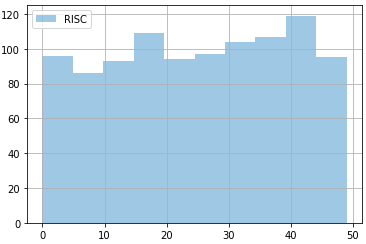
\includegraphics[scale=0.8]{Img/RngGrafico.png}
\end{figure}

% valori calcolati e tempo di exe
Un utilizzo del generatore di numeri casuali è un algoritmo di Monte Carlo. Il metodo di Monte Carlo è un'ampia classe di metodi computazionali basati sul campionamento casuale per ottenere risultati numerici.  In particolare si è utilizzato il metodo applicato al calcolo del pigreco.
Il metodo utilizzato funziona nel seguente modo:
\begin{itemize}
	\item[1] Genera due numeri casuali tra 0 e 1 che rappresentano le coordinate di un punto.
	\item[2] Applica il teorema di Pitagora, se supera uno allora il punto non appartiene alla circonferenza, altrimenti appartiene.
	\item[3] Ripeti i punti 1,2.
	\item[4] Calcola il valore del pigreco.
\end{itemize}


\begin{figure}[ht]
\centering
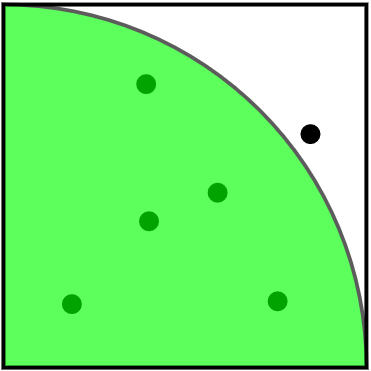
\includegraphics[scale=0.3]{Img/qCirc.png}
\caption{Esempio di coordinate generate casualmente}
\end{figure}

\begin{center}
$ \pi = 4 * \frac{Punti interni alla circonferenza}{Numero di ounti generati} $ 
\end{center}


\lstinputlisting[language=C,  style = Cstyle,  caption = {Funzione per il calcolo del pigreco con il metodo di Monte Carlo}, label = {Code:MonteCarloPi}]{PorzioniCodice/MonteCarloPi/MCPi.c}	

Inseguito vengono riportate le tabelle che rappresentano il tempo di esecuzione e il valore calcolato.

\begin{table}[ht]
\begin{tabular}{| l | c | c | c | c | c | c | c  | c |}
\hline
             & 1          & 2          & 3          & 4          & 5          & T.EXE Totale & MEDIA      & DEV.STD  \\ \hline
10\textasciicircum{}1  & 0,000008   & 0,000008   & 0,000006   & 0,000005   & 0,000006   & 0,000033     & 0,000007   & 0,000001 \\ \hline
10\textasciicircum{}2  & 0,000019   & 0,000019   & 0,000018   & 0,000018   & 0,000018   & 0,000092     & 0,000018   & 0,000001 \\ \hline
10\textasciicircum{}3  & 0,000141   & 0,000140   & 0,000141   & 0,000140   & 0,000140   & 0,000702     & 0,000140   & 0,000001 \\ \hline
10\textasciicircum{}4  & 0,001467   & 0,001501   & 0,001524   & 0,001362   & 0,001382   & 0,007236     & 0,001447   & 0,000072 \\ \hline
10\textasciicircum{}5  & 0,014029   & 0,014082   & 0,013851   & 0,013994   & 0,013971   & 0,069927     & 0,013985   & 0,000086 \\ \hline
10\textasciicircum{}6  & 0,138878   & 0,138625   & 0,138920   & 0,138916   & 0,138660   & 0,693999     & 0,138800   & 0,000145 \\ \hline
10\textasciicircum{}7  & 1,393739   & 1,387346   & 1,387775   & 1,387397   & 1,390657   & 6,946914     & 1,389383   & 0,002796 \\ \hline
10\textasciicircum{}8  & 13,881088  & 13,880401  & 13,882388  & 13,880326  & 13,880459  & 69,404662    & 13,880932  & 0,000869 \\ \hline
10\textasciicircum{}9  & 138,820115 & 138,830064 & 138,831942 & 138,863054 & 138,809745 & 694,154920   & 138,830984 & 0,019997 \\ \hline
10\textasciicircum{}10 & 195,756279 & 195,752334 & 195,733842 & 195,746235 & 195,755829 & 978,744519   & 195,748904 & 0,009329 \\ \hline
\end{tabular}
\caption{Tempi di esecuzione dell algoritmo}
\label{Tab:TimeExceMCPi}
\end{table}


\begin{table}[ht]
\begin{tabular}{|l|c|c|c|c|c|c|c|}
\hline
               & 1        & 2        & 3        & 4        & 5        & MEDIA    & DEV.STD  \\ \hline
10\textasciicircum{}1  & 3,600000 & 3,200000 & 2,400000 & 3,200000 & 3,200000 & 3,120000 & 0,438178 \\ \hline
10\textasciicircum{}2  & 2,840000 & 3,160000 & 3,040000 & 3,160000 & 3,000000 & 3,040000 & 0,132665 \\ \hline
10\textasciicircum{}3  & 3,100000 & 3,136000 & 3,236000 & 3,168000 & 3,192000 & 3,166400 & 0,052046 \\ \hline
10\textasciicircum{}4  & 3,160000 & 3,128000 & 3,157200 & 3,110400 & 3,156400 & 3,142400 & 0,022114 \\ \hline
10\textasciicircum{}5  & 3,134120 & 3,138920 & 3,145400 & 3,143120 & 3,143200 & 3,140952 & 0,004482 \\ \hline
10\textasciicircum{}6  & 3,140340 & 3,140840 & 3,145420 & 3,139996 & 3,143304 & 3,141980 & 0,002319 \\ \hline
10\textasciicircum{}7  & 3,142072 & 3,141478 & 3,142091 & 3,141413 & 3,141392 & 3,141689 & 0,000360 \\ \hline
10\textasciicircum{}8  & 3,141343 & 3,141380 & 3,141467 & 3,141383 & 3,141244 & 3,141363 & 0,000081 \\ \hline
10\textasciicircum{}9  & 3,141499 & 3,141617 & 3,141583 & 3,141508 & 3,141531 & 3,141548 & 0,000051 \\ \hline
10\textasciicircum{}10 & 3,141637 & 3,141616 & 3,141607 & 3,141607 & 3,141506 & 3,141595 & 0,000051 \\ \hline
\end{tabular}
\caption{Valori calcolati}
\label{Tab:ValueMCPi}
\end{table}

Le tabelle \ref{Tab:TimeExceMCPi} e \ref{Tab:ValueMCPi} mostrano i risultati in termini di valori calcolati e il tempo di esecuzione.  Le colonne indicano il valore dell i-esima prova mentre ogni riga identifica il numero di punti generati.

\section{Sorting}
Gli algoritmi di ordinamento sono una parte importante dell'elaborazione dei dati e sono ampiamente utilizzati in molti aspetti, ad esempio in crittografia e nella ricerca di informazioni. Esistono molti tipi di algoritmi di ordinamento e ognuno ha i suoi vantaggi e limiti. In informatica, l'algoritmo di ordinamento è solitamente classificato come segue.

\begin{itemize}
	\item La complessità temporale.  Si basano su quanti valori si ha da distribuire. Questi vengono indicati con n.Possiamo avere una prestazione buona come $\mathcal{O}(n\log{}n)$ oppure peggiori come $\mathcal{O}(n!)$.
	\item Memoria utilizzata.
	\item Stabilita ovvero se viene preservato l'ordine relativo dei dati con chiavi uguali all'interno dei valori da ordinare.
\end{itemize}

In base alle proprietà dei diversi tipi di dati, l'efficienza può essere migliorata scegliendo algoritmi di ordinamento appropriati. In questo capitolo verranno descritti quattro algoritmi di ordinamento e verranno analizzati comparandoli all esecuzione su raspberry. L'ordinamento a cui si fa riferimento nelle sezioni successive è un ordinamento di array da mettere in ordine non decrescente.

\subsection{Bubble sort}
Bubble sort è un semplice algoritmo di ordinamento. 
L'algoritmo funziona nel modo seguente:
\begin{itemize}
	\item Confronta gli elementi adiacenti, se il primo è maggiore del secondo, scambialo.
	\item Fai lo stesso confronto di prima dalla prima coppia all'ultima coppia. 
	\item Ripeti i 2 passaggi precedenti per tutti gli elementi tranne l'ultimo.
	\item Ripeti tutti i 3 passaggi precedenti finché non sono necessari elementi da scambiare.
\end{itemize}
L'efficienza dell algoritmo è basata sull' ordinamento dell array da ordinare. Nel caso migliore l'array è gia ordinato e , passandolo all algoritmo, esegue solo il punto 1 dall inizio alla fine. In contrario il caso peggiore è quando l'array si trova nell ordine non crescente.
\begin{table}[ht]
	\centering
	\begin{tabular}{lc}
              & Complessità \\
Caso peggiore &       $ \mathcal{O}(n^2)$      \\
Caso migliore &           $ \mathcal{O}(n)$   \\
\end{tabular}
	\caption{complessita bubble sort}
	\label{Tab:CompBubbleSort}
\end{table}

Di seguito viene riportato il codice (Code \ref{Code:BubbleSort}) dell'algoritmo e i tempi di esecuzione(Tab \ref{Tab:Tempi esecuzione Bubblesort}) secondo la dimensione dell array e la situazione iniziale dell array:
\lstinputlisting[language=C,  style = Cstyle,  caption = {Algoritmo bubble sort scritto in c}, label = {Code:BubbleSort}]{PorzioniCodice/Sorting/Bubble.c}	

\begin{table}[ht]
\centering
\begin{tabular}{| l | l | l | l |}
\hline
      & Caso peggiore & Caso migliore & Caso Generale \\ \hline
500   & 0.009426      & 0.004667      & 0.007156      \\ \hline
1000  & 0.037558      & 0.018877      & 0.028745      \\ \hline
5000  & 0.941429      & 0.470478      & 0.718178      \\ \hline
10000 & 3.784664      & 1.893387      & 2.889989      \\ \hline
20000 & 15.249109     & 7.639312      & 11.617705     \\ \hline
35000 & 46.744558     & 23.460390     & 35.640101     \\ \hline
50000 & 95.389578     & 47.888541     & 72.735791    \\ \hline
\end{tabular}
\caption{Tempi di esecuzione bubble sort}
\label{Tab:Tempi esecuzione Bubblesort}
\end{table}

\newpage
\subsection{Insertion sort}
L'arlogitmo consiste nel considerare un elemento alla volta, inserendo ciascuno nella posizione corretta tra gli elementi che sono stati ordinati. 
\begin{table}[ht]
	\centering
	\begin{tabular}{lc}
              & Complessità \\
Caso peggiore &       $ \mathcal{O}(n!)$      \\
Caso migliore &           $ \mathcal{O}(n)$   \\
Caso medio &  $ \mathcal{O}(n!)$\\
\end{tabular}
	\caption{complessita insertion sort}
	\label{Tab:CompInsertionSort}
\end{table}


\lstinputlisting[language=C,  style = Cstyle,  caption = {Algoritmo bubble sort scritto in c}, label = {Code:InsertionSort}]{PorzioniCodice/Sorting/Insertion.c}	

Come nel caso del bubble sort è riportato anche il tempo di esecuzione nel caso peggiore e migliore.

\begin{table}[ht]
\centering
\begin{tabular}{| l | l | l | l |}
\hline
           & Caso peggiore & Caso migliore & Caso Generale \\ \hline
500   & 0.005423      & 0.000028      & 0.002634      \\ \hline
1000  & 0.020836	    & 0.000055      & 0.010575      \\ \hline
5000  & 0.521686      & 0.000287     & 0.260862     \\ \hline
10000 & 2.103697      & 0.000645     & 1.048553      \\ \hline
20000 & 8.497346     & 0.001114      & 4.220421     \\ \hline
35000 & 26.066370     & 0.001928     & 12.969309     \\ \hline
50000 & 53.187672     & 0.002720   & 26.499820    \\ \hline

\end{tabular}
\caption{Tempi di esecuzione insertion sort}
\label{Tab:Tempi esecuzione InsertionSort}
\end{table}


\subsection{QuickSort}
L'algoritmo quicksort è un algoritmo ricorsivo del tipo divide et impera.L'algoritmo si basa:
\begin{itemize}
\item Scegli un pivot dagli elementi dell'array.
\item Ordina l' array.Se l'elemento è più grande del pivot, allora mettilo  dopo il pivot, altrimenti prima.
\item Ripetere questi due passaggi per i sottoarray finché ogni elemento non è nell'ordine corretto.
\end{itemize}

Il tempo di esecuzione nel caso peggiore di $\mathcal{O}(n!) $, il tempo di esecuzione medio di quicksort è $\mathcal{O}(n * \log{}n) $. In seguito viene mostrato l'implementazione 

\lstinputlisting[language=C,  style = Cstyle,  caption = {Algoritmo quick sort scritto in c}, label = {Code:QuickSort}]{PorzioniCodice/Sorting/Quick.c}	

\begin{table}[ht]
\centering
\begin{tabular}{| l | l  |}
\hline
            & Tempo \\ \hline
500   & 0.000273      \\ \hline
1000  & 0.000610      \\ \hline
5000  & 0.003813     \\ \hline
10000 & 0.008423      \\ \hline
20000 & 0.017266     \\ \hline
35000 & 0.032285     \\ \hline
50000 & 0.048096    \\ \hline

\end{tabular}
\caption{Tempi di esecuzione quick sort}
\label{Tab:Tempi esecuzione QuickSort}
\end{table}

\subsection{Heap sort}
L'heapsort è un algoritmo di ordinamento iterativo l'implementazione utilizzata è in-place.

\lstinputlisting[language=C,  style = Cstyle,  caption = {Algoritmo heap sort scritto in c}, label = {Code:HeapSort}]{PorzioniCodice/Sorting/Heap.c}	

\begin{table}[ht]
\centering
\begin{tabular}{| l | l  |}
\hline
            & Tempo \\ \hline
500   & 0.000569      \\ \hline
1000  & 0.001272      \\ \hline
5000  & 0.008016     \\ \hline
10000 & 0.017815      \\ \hline
20000 & 0.041886     \\ \hline
35000 & 0.083366     \\ \hline
50000 & 0.128863    \\ \hline

\end{tabular}
\caption{Tempi di esecuzione heap sort}
\label{Tab:Tempi esecuzione HeapSort}
\end{table}

Come mostrato dai grafici \ref{Fig:AllSort} i risultati mostrano che il peggior algoritmo è il bubblesort mentre il migliore è quicksort.  Risultato poco notevole, nella sezione successiva un confronto più significativo.

\begin{figure}[ht]
     \centering
     \begin{subfigure}[t]{0.45\textwidth}
         \centering
         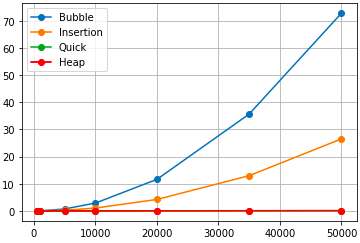
\includegraphics[width=\textwidth]{Img/GraficiSorting/AllSorting.png}
         \caption{Bubblesort insertionsort, heapsort e quicksort}
         \label{Fig:AllSortingAlg}
     \end{subfigure}
     \hfill
     \begin{subfigure}[t]{0.45\textwidth}
         \centering
         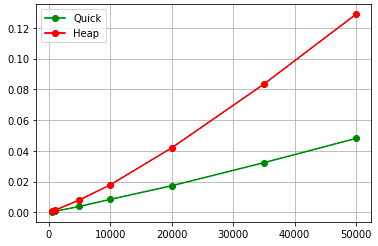
\includegraphics[width=\textwidth]{Img/GraficiSorting/QHSorting.png}
         \caption{Quicksort e Heapsort}
         \label{Fig:QHSort}
     \end{subfigure}

   \caption{Algoritmi di oridinamento a confronto}
   \label{Fig:AllSort}
\end{figure}


\subsection{Confronto Sorting}
In questa sezione vengono visualizzati i risultati a confronto. Per prima cosa iniziamo con confrontare i risultati con l'esecuzione su MacBook.

\begin{figure}[ht]
     \centering
     \begin{subfigure}[t]{0.49\textwidth}
         \centering
         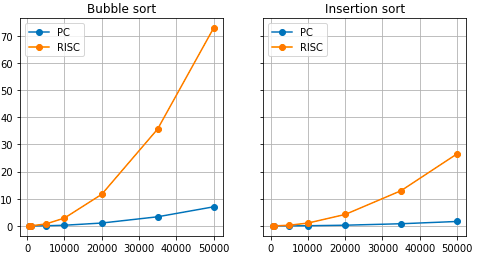
\includegraphics[width=\textwidth]{Img/GraficiSorting/BubbleInsert.png}
       
     \end{subfigure}
     \hfill
     \begin{subfigure}[t]{0.49\textwidth}
         \centering
         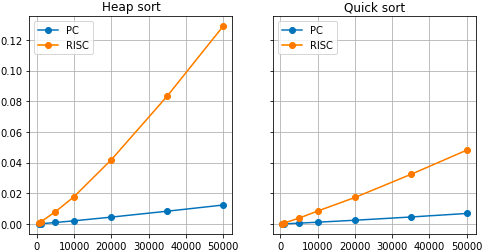
\includegraphics[width=\textwidth]{Img/GraficiSorting/HeapQuick.png}
        
     \end{subfigure}

   \caption{Algoritmi di oridinamento a confronto eseguiti su PC e su RISC-V}
   \label{Fig:AllSort_PC}
\end{figure}
	
	
	\begin{table}[ht]
		\centering
		\begin{tabular}		{| l | c | c | c | c |}
		\hline
		      & Bubblesort & Insertionsort & Heapsort & Quicksort \\ \hline
500   & 0.000491      & 0.000196      & 0.000057 & 0.000052     \\ \hline
1000  & 0.001871	    & 0.000723      & 0.000145 & 0.000080     \\ \hline
5000  & 0.055505      & 0.016859     & 0.000975  & 0.000544   \\ \hline
10000 & 0.247916      & 0.066411     & 0.002083 & 0.001164     \\ \hline
20000 & 1.056383   & 0.261627      & 0.004485  & 0.002441   \\ \hline
35000 & 3.359662     & 0.800075     & 0.008340  & ;0.004557   \\ \hline
50000 & 7.019640     & 1.633171   & 0.012359  & 0.006857  \\ \hline

		\end{tabular}
		\caption{Tempi di esecuzione degli algoritmi di sorting su PC}
		\label{Fig:PcSort}
	\end{table}

La tabella \ref{Fig:PcSort} mostra i tempi di esecuzione degli algoritmi di ordinamento eseguiti sul PC. 
Un altro confronto lo possiamo fare con Raspberry pi \footnote{Il modello utilizzato è il modello Raspberry model B mostrato in figura \ref{fig:RaspberryB} }.

\begin{figure}[ht]
\centering
	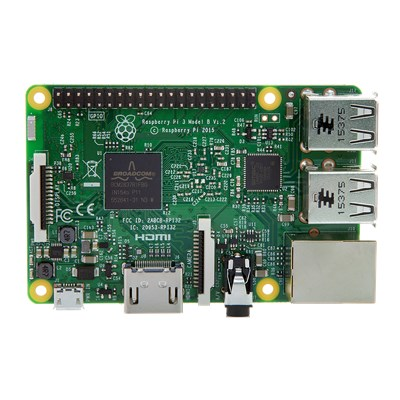
\includegraphics[scale=0.5 ]{RBTop.jpeg}
	\caption{Vista superiore Raspberry model B}
	\label{fig:RaspberryB}
\end{figure}

Il Raspberry Pi utilizzato è Raspberry Pi model B. La board datata 2013 è stata sviluppata come board scolastica e successivamente applicata a molti contesti come nel mondo embedded.
Con la dimensione di una carta di credito il Raspberry ha una RAM di 512 MB e una CPU da 700 MHz,due porte USB (Universal Serial Bus) e un'Ethernet da 100 MB porta. In aggiunta a ciò, ci sono pin di input/output (GPIO) per uso generico per collegare alcuni hardware.  La tabella \ref{Tab:RaspSorting} mostra i tempi di esecuzione degli algoritmi di ordinamento eseguiti su Raspberry \cite{Rasp}.

\begin{table}[ht]
		\centering
		\begin{tabular}		{| l | c | c | c | c |}
		\hline
		      & Bubblesort & Insertionsort & Heapsort & Quicksort \\ \hline
500   & 0.020337      & 0.004877      & 0.000825 & 0.000511     \\ \hline
1000  & 0.078527	    & 0.020353      & 0.001894 & 0.001141     \\ \hline
5000  & 2.030446      & 0.045018     & 0.013863  & 0.009072   \\ \hline
10000 & 8.535436      & 1.874295     & 0.027671 & 0.018542     \\ \hline
20000 & 34.733894   & 7.842624      & 0.058596  & 0.038194   \\ \hline
35000 & 117.622606     & 24.076289     & 0.114716  & 0.082891   \\ \hline
50000 & 250.008917     & 51.757841   & 0.210807  & 0.157344  \\ \hline

		\end{tabular}
		\caption{Tempi di esecuzione Raspberry Pi B}
		\label{Tab:RaspSorting}
			\end{table}

\begin{figure}[ht]
     \centering
     \begin{subfigure}[t]{0.49\textwidth}
         \centering
         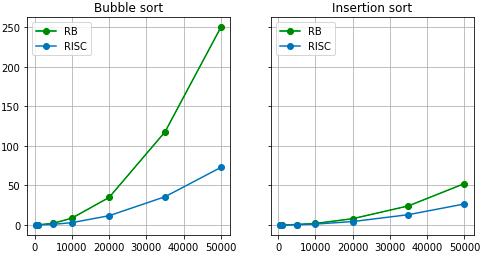
\includegraphics[width=\textwidth]{Img/GraficiSorting/BISort_RB.png}
        
     \end{subfigure}
     \hfill
     \begin{subfigure}[t]{0.49\textwidth}
         \centering
         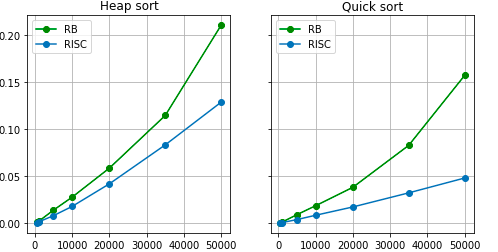
\includegraphics[width=\textwidth]{Img/GraficiSorting/HQSort_RB.png}
         
     \end{subfigure}

   \caption{Algoritmi di oridinamento a confronto eseguiti su Raspberry e su RISC-V}
   \label{Fig:AllSort_RB}
\end{figure}

I grafici \ref{Fig:AllSort_RB} mostrano i tempi di esecuzione degli algoritmi di sorting comparati tra Rasberry e RISC-V. In ogni grafico si vede che il tempo di esecuzione è migliore su RISC-V. Prendendo in considerazione il Bubblesort nel caso con 50000 elementi la board con processore RISC-V è 4 volte piu veloce del raspberry in altri casi, come ad esempio per heap sort, il miglioramente di RISC-V è 1.6 rispetto a Raspberry. 

\section{BackTracking}
Un altro problema che si puo affrontare è il problema del backtracking, ovvero quella tecnica per cui è necessario tornare su dei passi precedenti per trovare la soluzione al problema. Il primo programma utilizzato è un solutore di sudoku.
I primi sudoku sono di difficoltà crescente mentre gli utlimi sono impossibili, uno impossibile per costruzione (sbagliato dalla partenza) , e l'altro impossibile completarlo.
\begin{table}
\centering
\begin{tabular}{  |l | c | c |}
\hline
	& RISC-V & PC \\ \hline
	1 & 0.004475 & 0.000384  \\ \hline
2 & 0.055382 &0.004791           \\ \hline
3 & 0.000282 &0.000026  \\ \hline
4 & 0.048991 &0.005037  \\ \hline
5 & 0.297553 &0.025939  \\ \hline
6 & 1.488701 &0.122498  \\ \hline
7 & 6.548320 &0.534505  \\ \hline
8 & 0.001508 &0.000241  \\ \hline
Vuoto & 0.001680 & 0.000267  \\ \hline
\end{tabular}

	\caption{Tempi di esecuzione del solutore di sudoku}
	\label{Tab:SudoSolver}
	\end{table}
	
Il secondo problema che utilizza il backtracking è un solutore di labirinti.

\begin{table}
\centering
\begin{tabular}{  | l | c | c |}
\hline
 & RISC & PC  \\ \hline
maze0 & 0.000102 & 0.000007  \\ \hline
maze1 & 0.005261 & 0.000235  \\ \hline
maze2 &0.009123 & 0.000371  \\ \hline
\end{tabular}

	\caption{Tempi di esecuzione del solutore di labirinti}
	\label{Tab:MazeSolver}
	\end{table}



%--------

\chapter{Conclusione}
In questa tesi si sono fatti alcuni test su RISC-V.  Si è controllato aspetti comuni come le operazioni aritmetiche e alcuni algoritmi di ordinamento.  Si è guardato il codice assembly generato dal compilatore e osservato le implementazioni delle varie operazioni comparandolo con altri codici assembly. Oltre alla comparazione con altri codici assembly si è comparato con diversi livelli di ottimizzazione.  Per ogni operazione è stato calcolato il tempo di esecuzione.
Infine sono stati utilizzati degli algoritmi di ordinamento i cui risultati sono stati confrontati con un Raspberry.

Questa tesi analizza solo alcuni aspetti di RISC-V, terminato questo lavoro di tesi vorrei sottolineare che non si tratta di un lavoro concluso, ma un punto di partenza per possibili approfondimenti futuri.  




%\addcontentsline{toc}{chapter}{Bibliografia}

\printbibliography

\end{document}
